\documentclass[12pt,a4paper]{article}
\usepackage{fullpage}
\usepackage[margin=2cm]{geometry}
\usepackage{amsmath}
\usepackage{subfig}
\usepackage{graphicx}
\usepackage[justification=centering]{caption}
\begin{document}
\title{Landmarks prediction on Beetle anatomical by applying Convolutional Neural Network }
\author{LE Van Linh}
\date{\today}
\maketitle
\begin{abstract}
	In morphometric studies, landmarks are regarded as one of important properties to analyze the object's shape. Especially in biology, collecting complete landmarks give us the information of the oganism. From that, the biologists can study the complex interactions between evolution of the oganism and environment factors. In the context of this study, we focus on one of the most common insect of North-Western France, Carabidae (Beetle). Landmarking manually will be a time-consuming process. In order to investigate the posibility of automatic identify the landmarks on Beetles, we propose a convolutional neural network (CNN) to predict the landmarks on the parts of Beetle: pronotum, head, and body. The proposed model will witnessed on the datasets includes $293$ images (for each part) in different sizes. The experiments will be done in two directions: training the model from scratch and using fine-tuning. During the experiments, the coordinates of automatic landmarks will be evaluated by comparing with the manual coordinates, which are given by the biologists.
\end{abstract}
\section{Introduction}
Morphometric landmarks are important features in biological investigations. They are use to analyze the shape of the organisms. Depending on the organisms, the number of landmarks on their shapes is different. When we consider the position of the landmarks with the shape, most of landmarks are located on the edges, for example, the landmarks on wings of Drosophila fly \cite{.}. Besides, we can also see the landmarks which stayed inside the anatomical part, i.e, landmarks on pinna of human ears \cite{.}. Currently, the landmarks are set manually by the biologsits. However, landmarking manually will be a time-consuming process and difficult to pre-process. Consequently, a process that proposed automatically the coordinates of landmarks could be interested.

In image processing, segmentation is a most often step of the methods. In some cases, the object of
interest is easy to extract and can be analyzed with the help of a lot of very well-known image analysis procedures. The result of segmentation step is very useful for many purposes. Depending on purpose of the applications, the object can be segmented or un-segmented before continuing the futher steps. Landmarks setting is no different. In a previous study \cite{.}, we have analyzed two parts of beetle: left and right mandibles. These parts are easy to segment. In that work, we have applied a set of algorithm based on segmentation, image alignment and SIFT \cite{.}. 
\section{Dataset}
The data includes images in three sets of the beetle: pronotum, body, and head (Fig.\ref{figdata}). Each dataset includes 293 color images. For each dataset, the images are divided into two subsets: training and validation (called training set) include 260 images, and the testing set has 33 images. To have enough images for training process, the training sets have been combined together. Then, the training dataset was enlarged to $5460$ images ($1820 \times 3$) following the way that we change the values of pixels on the images. At this time, we have enough the images for training. However, another problem has occurred: the number of landmarks of each part is different: $8$ landmarks on pronotum part, $11$ landmarks on the body part, and $10$ landmarks on the head part. We see that the trained model will be fine-tuned on pronotum dataset. So, we kept the number of the landmark on pronotum as a reference and we suppress some landmarks on body and head part. Specifically, we have removed \textit{three} landmarks on the body part ($1^{st}, 6^{th}, 9^{th}$) and \textit{two} landmarks on the head part ($5^{th}, 6^{th}$).
\begin{figure}[h!]
\centering
\subfloat{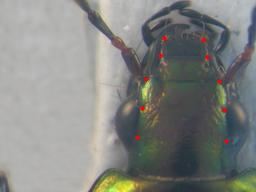
\includegraphics[scale=0.5]{./images/ftete}}~~
\subfloat{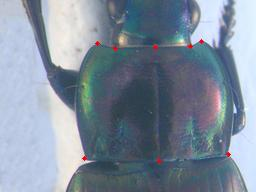
\includegraphics[scale=0.5]{./images/fpronotum}}~~
\subfloat{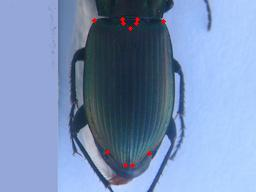
\includegraphics[scale=0.5]{./images/felytre}}\\
\subfloat{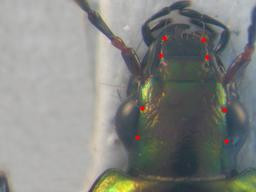
\includegraphics[scale=0.5]{./images/ftete2}}~~
\subfloat{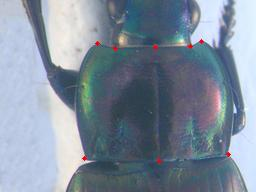
\includegraphics[scale=0.5]{./images/fpronotum}}~~
\subfloat{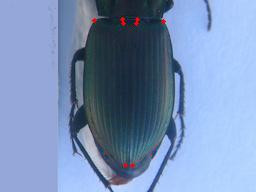
\includegraphics[scale=0.5]{./images/felytre2}}
\caption{The dataset images. \textit{Top row}: The images with their manual landmarks. \textit{Bottom row}: The training images (some landmarks have been removed on head and body parts)}
\label{figdata}
\end{figure}
\section{The model}
In this study, we use the model that we have used to train on pronotum dataset. 
The network consists on three repeated-structure of a convolutional layer followed by a maximum pooling layer and dropout layer. The depth
of convolutional layers increases from $32, 64,$ and $128$ with
different size of the filter kernel: $3 \times 3, 2 \times 2$, and $2 \times 2$.
All the kernels of pooling layers have the same size of $2 \times 2$. The dropout probability values used for dropout layers are $0.1, 0.2,$ and $0.3$.
Then, three full connected layers have been added to the
network. A dropout layer with probability of $0.5$ was added between the first two full connected layers. The outputs of the full connected layers are $1000, 1000,$
and $16$, respectively. The output of the last full-connected
layer corresponds to $8$ landmarks (x and y coordinates) which
we would like to predict (Fig. \ref{1Econv}). 
\begin{figure}[h!]
	\centering
	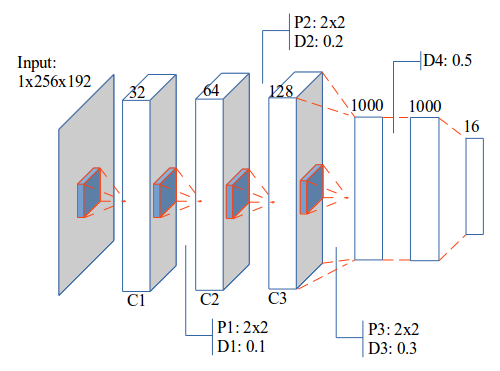
\includegraphics[scale=0.45]{images/architecture3}
	\caption{The architecture of CNN model}
	\label{1Econv}
\end{figure}\\
The parameters of CNN are shown in Table.x.
\begin{table}[h!]
	\centering
	\begin{tabular}{l l l}
	Parameter & Initial value & End value \\ \hline
	Epochs & 10000 &  \\ \hline
	Training batch size & 128 & \\ \hline
	Testing batch size & 128 & \\ \hline
	Learning rate & 0.03 & 0.0001 \\ \hline
	Momentum & 0.9 & 0.9999 \\ \hline
	\end{tabular}
	\caption{The network parameters in proposed model}
	\label{model2parameters}
\end{table}
\section{Experiments}
\subsection{Training on three parts of beetle}
The dataset includes $5460$ images was trained on the model with $10000$ epochs\footnote{An epoch is a single pass through the full training set}. The images are randomly divided into training set and validation set followed the ratio $6:4$. The learning rate began at $0.03$ and decreased to $0.00001$ during training. In vice versa, the momentum started at $0.9$ and increasing to $0.999$ at the end of the training process. 

Fig.\ref{figlossallparts} shows the losses during training process. At the beginning, the validation loss is always higher than the tranining loss, but from the $2000^{}$ epochs, the training loss begins stable while the validation loss continue to decrease. At the end of training, the losses values are $0.00029$ and $0.00009$ for training and validation, respectively.

\begin{figure}[h!]
	\centering
	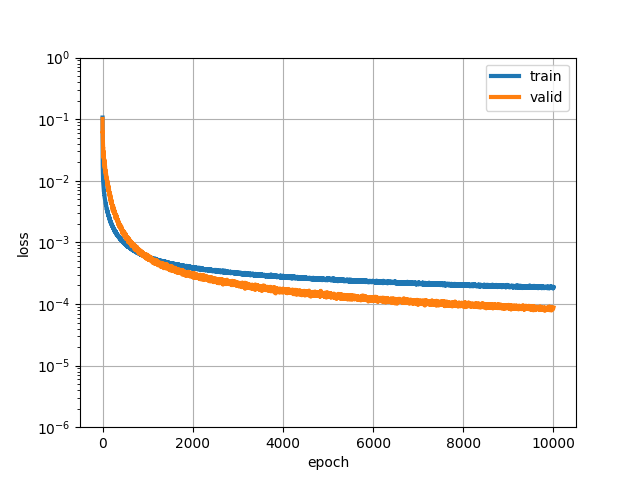
\includegraphics[scale=0.6]{images/all_parts_10000epochs}
	\caption{The losses during training on the images of three parts}
	\label{figlossallparts}
\end{figure}

Fig.\ref{figtestallparts} shows the predicted landmarks on some images in test set.
\begin{figure}[h!]
	\centering
	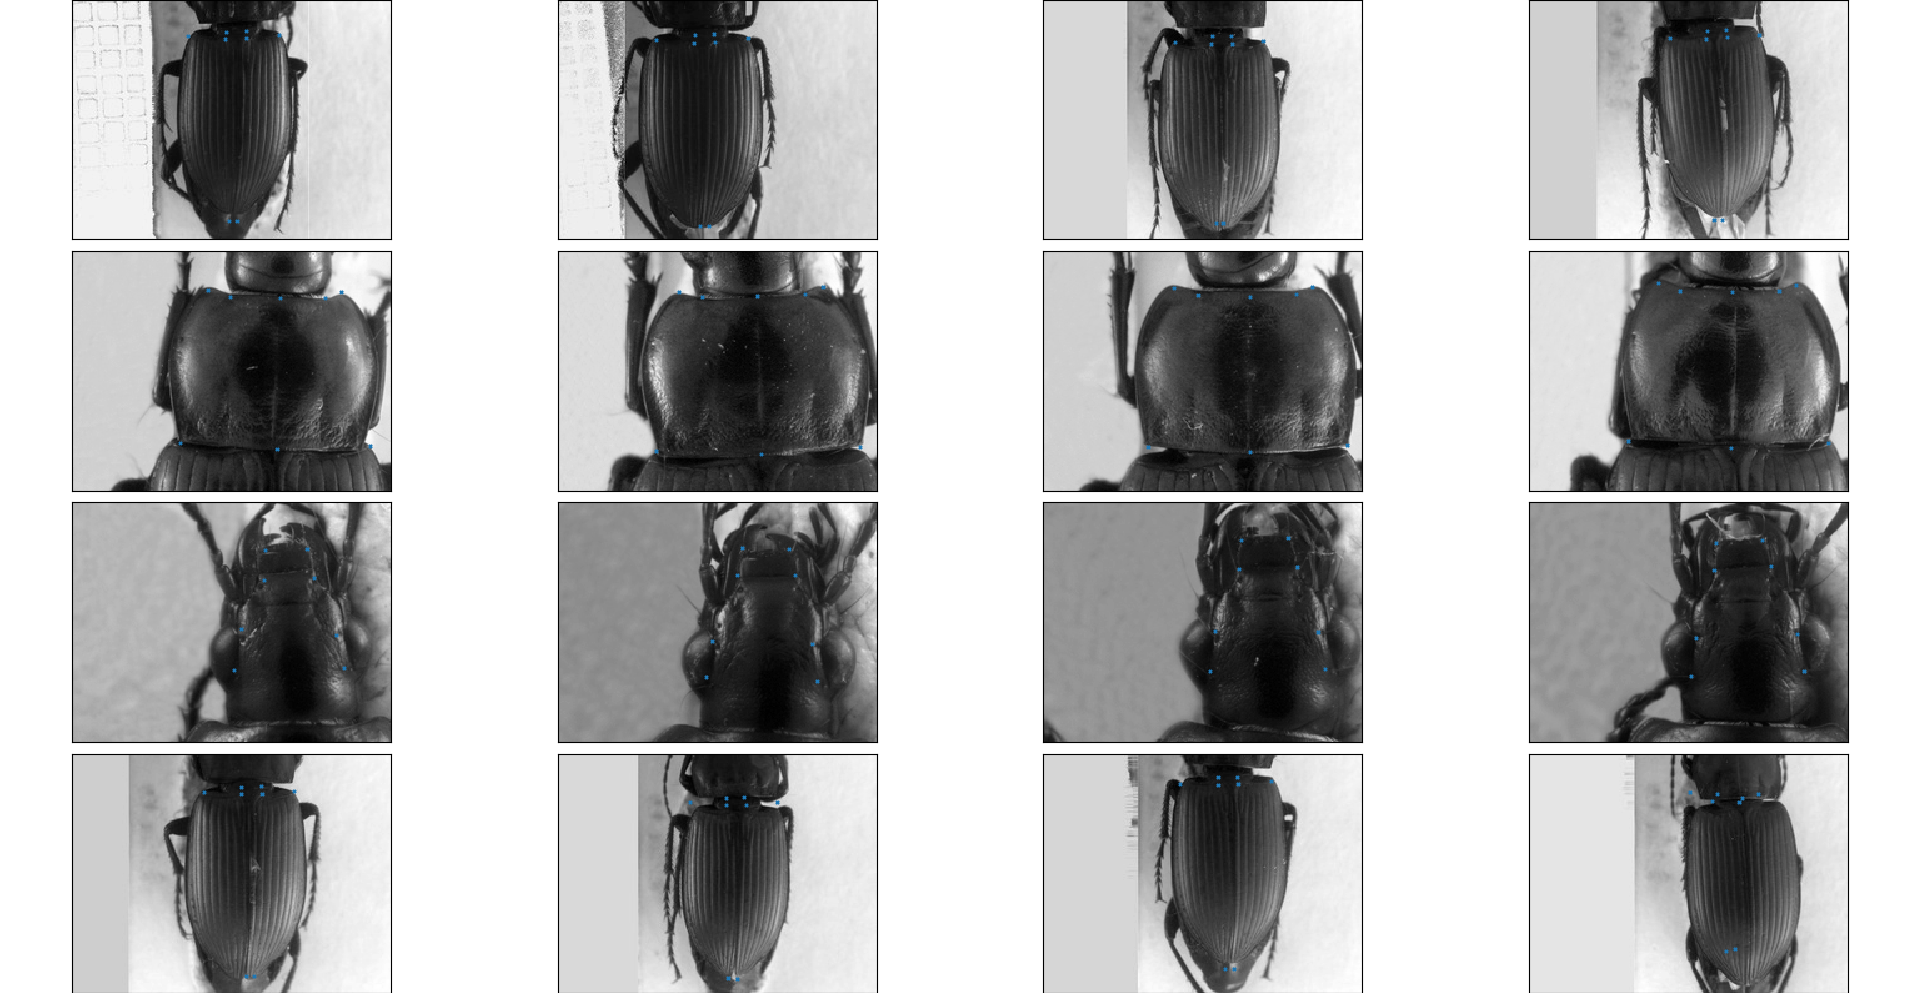
\includegraphics[scale=0.53]{images/all_parts_10000epochs_test}
	\caption{The blue points present for the predicted landmarks on the images in test set}
	\label{figtestallparts}
\end{figure}
\subsection{Fine-tuning on pronotum dataset}
The trained model have been continued to fine-tune \cite{yosinski2014transferable} with pronotum dataset. To get all predicted landmarks for the pronotum images, a scenario to choose the test images is executed. For each round, we have chosen 33 images for the test set, the remaining images have been put to training test. Table.\ref{finetuningloss} shows the losses during fine-tuning on different dataset of pronotum images.

\begin{table}[h!]
	\centering
	\begin{tabular}{l l l}
	Round & Training loss & Validation loss \\ \hline
	1 & 0.00019 & 0.00009  \\ \hline
	2 & 0.00018 & 0.00010 \\ \hline
	3 & 0.00018 & 0.00010 \\ \hline
	4 & 0.00019 & 0.00008 \\ \hline
	5 & 0.00019 & 0.00009 \\ \hline
	6 & 0.00018 & 0.00008 \\ \hline
	7 & 0.00019 & 0.00008 \\ \hline
	8 & 0.00018 & 0.00006 \\ \hline
	9 & 0.00018 & 0.00009 \\ \hline
	\end{tabular}
	\caption{The losses during fine-tuning model}
	\label{finetuningloss}
\end{table}

Fig.\ref{figfintuning} shows an example of the losses during fine-tuning and corresponding predicted landmarks on the test set.

\begin{figure}[h!]
\centering
\subfloat[Training losses and validation loss]{\label{model1loss}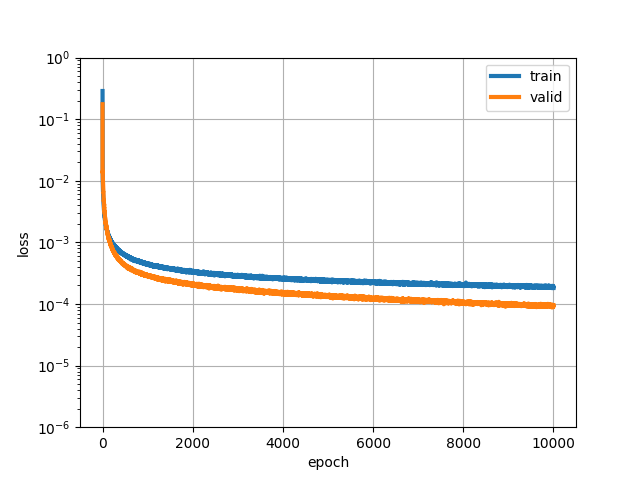
\includegraphics[width=0.3\textwidth]{./images/pronotum_fine_tuning_v11}}~~
\subfloat[A pronotum with predicted landmarks]{\label{model1test}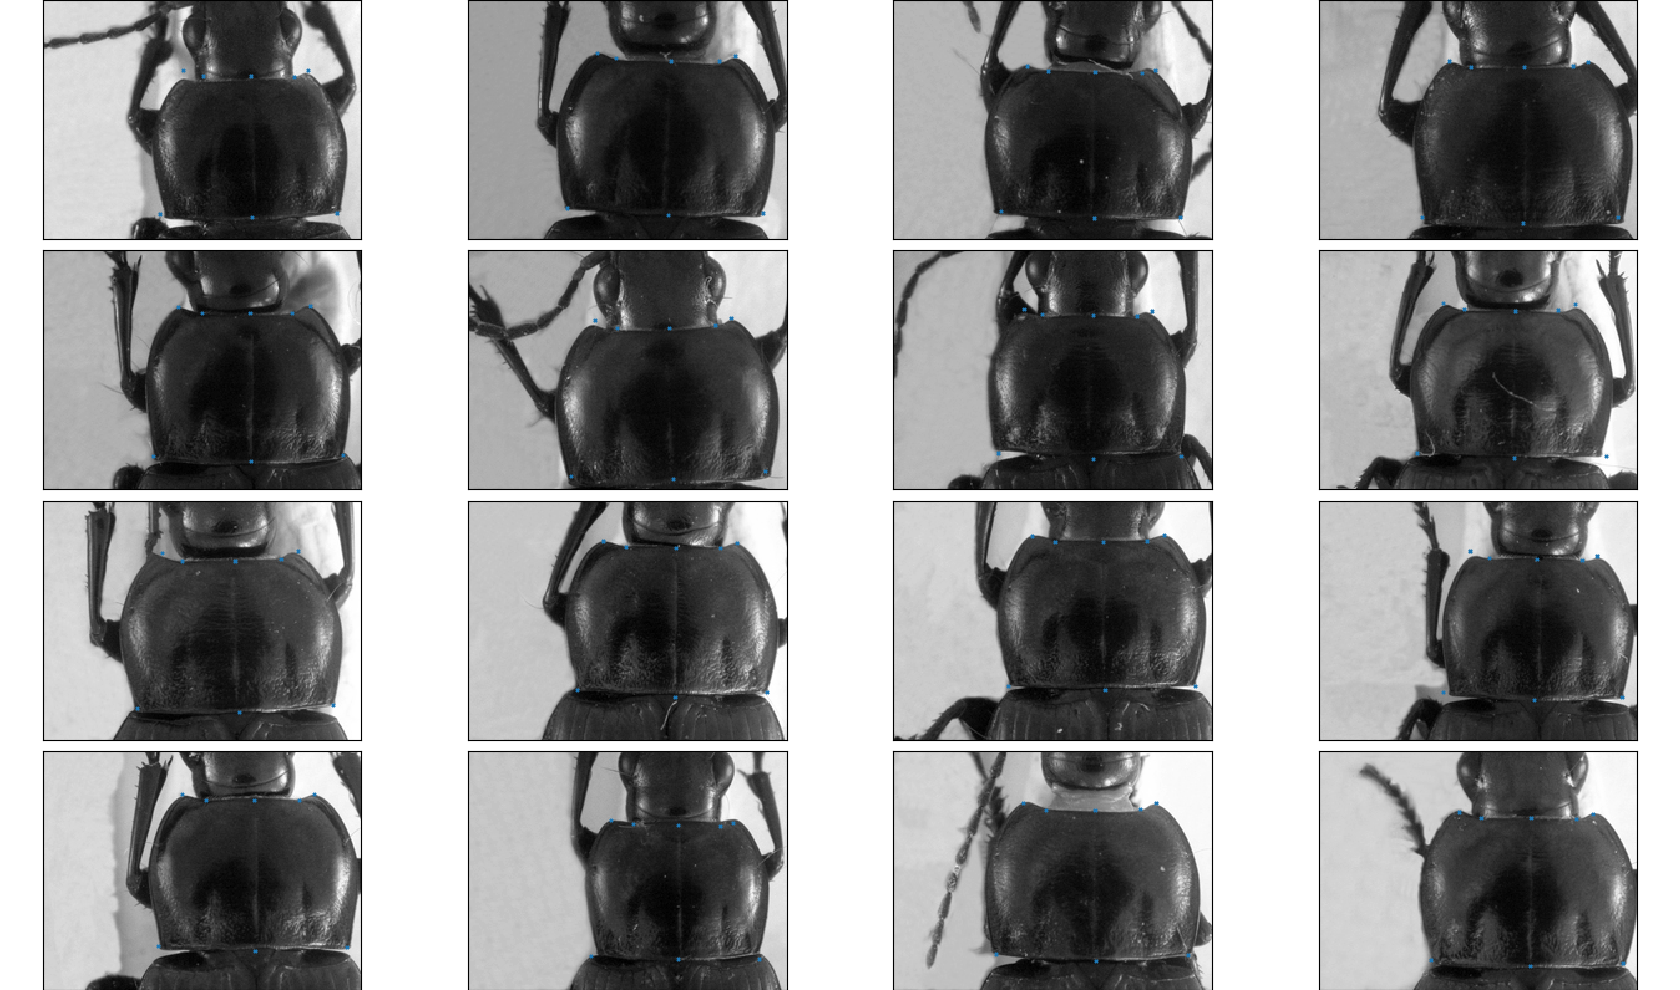
\includegraphics[width=0.7\textwidth]{./images/pronotum_fine_tuning_v11_test}}
\caption{An result example when fine-tuning the trained model on pronotum dataset}
\label{figfintuning}
\end{figure}
After fine-tuning, the predicted landmarks of all images are provided. To evaluate the effects of fine-tuning, we calculated the distance between the predicted landmarks and corresponding manual landmarks. A statistic on the distance of each landmarks is also computed. 

Table.\ref{tab2} shows the average error distance given by each landmark. The values in \textbf{Distance 1} and \textbf{Distance 2} columns present for the average distance of all landmark when the pronotum images were trained from scratch and fine-tuning, respectively. From the Table. \ref{tab2}, the result from fine-tuning is significantly improved ($\sim 38\%$) 
\begin{table}[htbp]
\begin{center}
\begin{tabular}{|c|p{2.5cm}|p{2.5cm}|}
\hline
\textbf{$\#$Landmark} & \textbf{Distance 1} & \textbf{Distance 2} \\ \hline
1 & 4.002 & 2.486  \\ \hline
2 & 4.4831 & 2.720  \\ \hline
3 & 4.2959  & 2.652 \\ \hline
4 & 4.3865  & 2.771 \\ \hline
5 & 4.2925  & 2.487 \\ \hline
6 & 5.3631  & 3.049 \\ \hline
7 & 4.636  & 2.684 \\ \hline
8 & 4.9363  & 2.871 \\ \hline
\end{tabular}
\caption{The average error distance per landmark.}
\label{tab2}
\end{center}
\end{table}

\section{Conclusions}
A CNN model has been trained on a dataset that includes the images of three parts of beetle. The trained model then has been fine-tuned with the pronotum dataset. Comparing the losses when we trained the pronotum from scratch, the losses during fine-tuning has been improved $40\%$ on validation test. Besides, the coordinates of predicted landmarks are also more accuracy than the last result (training from scratch) (Table.\ref{tab2}). From the result, we can see that fine-tuning has affected to the results from CNN. However, the effects still limits in our case. The experiments of the techniques on fine-tuning need to do to reach to the result as we expect.
\bibliographystyle{unsrt}
\bibliography{includes/references}

\end{document}
